\section{Auswertung}

\subsection{Berechnung der Vertikalkomponente des Erdmagnetfeldes}

Der Strom $I_\text{vert}$, welcher durch die Spule zum Ausgleich der Vertikalkomponente des Erdmagnetfeldes fließt, kann aus den Umdrehungen des Ganiometers berechnet
werden. Anschließend wird das resultierende Magnetfeld mit der Formel
\begin{equation}
  B= \mu_0 \cdot  \frac{8}{\sqrt {125}}\cdot \frac{I\cdot N}{R}
  \label{eq:Hholz}
\end{equation}
bestimmt. Es ergibt sich für die Vertikalkomponente des Erdmagnetfelds ein Wert von
\begin{equation*}
  B_\text{vert. Erdmagnetfeld}=3,525\cdot 10^{-5}\,\text{T}.
\end{equation*}

\subsection{Berechnung der Horizontalkomponente des lokalen Erdmagnetfeldes sowie der Landé-Faktoren}
Die Ströme $I_1$ und $I_2$, die durch die Horizontalfeldspule und die Sweep-Spule fließen, werden aus den Umdrehungen der Ganiometer berechnet.
Aus diesen werden die Feldstärken der durch die Spulenströmen erzeugten Magnetfelder mit Formel \eqref{eq:Hholz}
berechnet.
Die berechneten Magnetfelder werden nun gegen die Frequenz $\nu$ aufgetragen.
Dies ist in Abbildung \ref{abb:graph} zu sehen.
Um nun die Landé-Faktoren $g_F$ und die Horizontalkomponente des Erdmagnetfeldes $B_\text{horz. Erdmagnetfeld}$ zu bestimmen, werden für beide Isotope eine lineare Ausgleichsrechnung der Form
\begin{equation}
  B=\underbrace{\frac{4\pi \mu_0}{e_0g_F}}_{a_i}\cdot \nu+B_\text{horz. Erdmagnetfeld}
\end{equation}
durchgeführt.
Diese Ausgleichsgeraden sind ebenfalls in Abbildung \ref{abb:graph} zu sehen.
Für die Horizontalkomponente des Erdmagnetfeldes ergibt sich ein gemittelter Wert von
\begin{equation}
  B_\text{horz. Erdmagnetfeld}=(2,19\pm0,05)\cdot 10^{-5}\,\text{T}.
\end{equation}
Aus den beiden Steigungen ergeben sich die Landé-Faktoren
\begin{equation}
  g_{F,1}=0,499\pm0,004
\end{equation}
und
\begin{equation}
  g_{F,2}=0,333\pm0,002.
\end{equation}

%gj
%2.0023
%I1
%1.506+/-0.014
%I2
%2.510+/-0.017

\begin{figure}[H]
 \centering
 \includegraphics[width=12cm]{graph.pdf}
 \caption{Horizontalkomponente des $B$-Feldes in Abhänigkeit der Frequenz}
 \label{abb:graph}
\end{figure}

\subsection{Berechnung der Kernspins $I$ der beiden Isotope}
Mit der Formel blaaaaaaaaaaaaaaa lässt sich der Faktor $g_J$ für den hier vorliegenden Fall $J=\frac{1}{2}$, $S=\frac{1}{2}$ zu $g_J=2,0023$ berechnen.
Da zudem $F=I+J$ gilt, kann die Formel blaaaaaaaaaaaaaaaaaaa2 nach dem Kernspin $I$ umgeformt werden:
\begin{equation}
I_\pm=\frac{g_J-4g_F}{4g_F}\pm \sqrt{\left(\frac{g_J-4g_F}{4g_F}\right)^2-\frac{3}{4}\left(1-\frac{g_J}{g_F}\right)}.
\end{equation}
Da physikalisch nur positive Ergebnisse für den Kernspin sinnvoll sind, werden die Kernspins der beiden Isootope über $I_+$ zu
\begin{equation}
I_1=1,51\pm0,1\approx \frac{3}{2}
\end{equation}
und
\begin{equation}
  I_2=2,51\pm0,2\approx \frac{5}{2}
\end{equation}
berechnet.

\subsection{Bestimmung des Isotoenverhältnisses}

In Abbildung \ref{abb:oszi1} sind die Amplituden der Resonanzen bei $100\,\text{kHz}$ zu erkennen. Um die Amplituden besser ablesen zu können, ist der Ausschnitt
in Abbildung \ref{abb:oszi2} noch einmal größer dargestellt. Für den ersten Peak ergibt sich eine Amlitude von 12 Einheiten, für den zweiten etwas größeren
Peak eine Amplitude von 20 Einheiten. Mit Formel \eqref{eq:verhaeltnis} ergibt sich das Verhältnis
\begin{equation}
  \frac{\gamma_{85}}{\gamma_{87}}=\frac{5}{3}\approx 1,667.
\end{equation}
Der Literaturwert kann aus dem Verhältnis\cite{isotop} der Anteile bestimmt werden und beträgt
\begin{equation}
  \frac{\text{Anteil}~ \ce{^{85}Rb}}{\text{Anteil}~ \ce{^{87}Rb}}=\frac{72,12\%}{27,83\%} \approx 2,593.
\end{equation}

\begin{figure}[H]
 \centering
 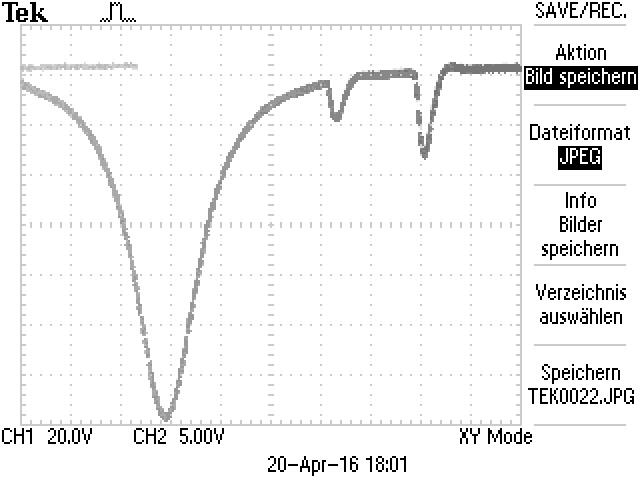
\includegraphics[width=12cm]{TEK0022.jpg}
 \caption{}
 \label{abb:oszi1}
\end{figure}


\begin{figure}[H]
 \centering
 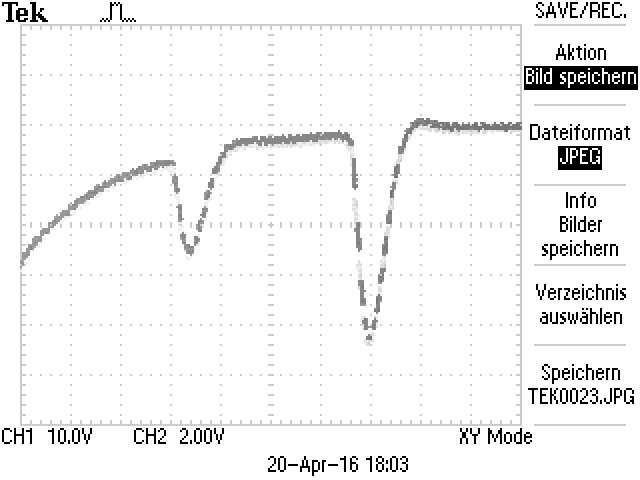
\includegraphics[width=12cm]{TEK0023.jpg}
 \caption{}
 \label{abb:oszi2}
\end{figure}


\subsection{Quadratischer Zeeman-Effekt}

Die Berechnung des quadratischen Zeeman-Effekts ergibt Ergebnisse mit der Potenz $10^{-28}$. Da diese Werte so klein sind, hat der quadratische Zeeman-Effekt keine
Auswirkung auf die Ergebnisse des Versuches. Er muss somit nicht bei der Auswertung betrachtet werden.
